\documentclass[11pt,a4paper,oneside]{article}
\usepackage[latin1]{inputenc}
\usepackage{amsmath}
\usepackage{amsfonts}
\usepackage{amssymb}
\usepackage{graphicx}
\usepackage{color}
\usepackage {tikz}
\usepackage{fancyvrb}
\usetikzlibrary {er}
\usepackage[left=2.00cm, right=2.00cm, top=1.00cm]{geometry}
\graphicspath{{./}}
\fvset{tabsize=4}

\begin{document}
	\title{DS 255 - System Virtualization \\ Assignment V - Process Virtual Machines}
	\author{Shriram R. \\ M Tech (CDS) \\ 06-02-01-10-51-18-1-15763}
	\maketitle	
	
	\begin{enumerate}
		\item With regard to compatibility frameworks, isomorphism focusses on the equivalence of mapped states between the guest and the host and the operation that transforms the state in the guest and the host. Isomorphism establishes an one-to-one mapping between the states and makes them equivalent at the points of control transfer between emulating user instructions and the host. This is illustrated in the following figure,		
				\begin{center}
				   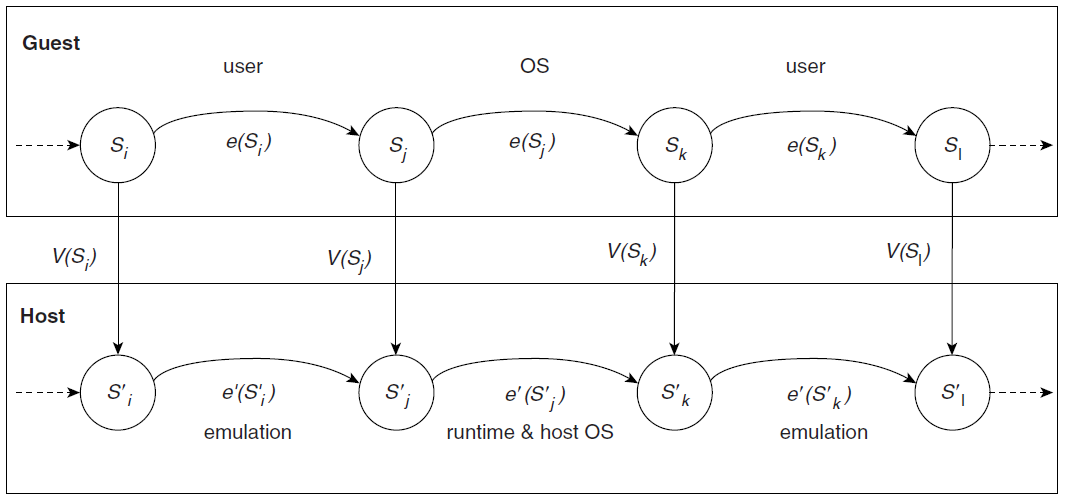
\includegraphics[scale=0.4]{1.png}
				\end{center}
		Isomorphism is necessary to establish the accuracy in emulating the guest's behaviour on the host platform as compared with its behaviour on the native platform. It also enables transparency during the emulation process. Another consequence is that the state equivalence has to be maintained only during points of control transfer (Trap/System Call) and not necessarily at all times. This allows for flexibility in terms of code reorganization and optimization. 
		
		\item 
		
		\item The compatibility aspects are met in Same OS-ISA process VMs as follows,
			\begin{enumerate}
				\item Two-level state : 
				\item Traps : 
				\item Register states : It is possible to have consistent register mapping since the ISAs are same. If no code reordering is done during translation/optimization, the source register state can be recovered from target at any point in execution
				\item Memory state : If code reordering is done as part of binary optimization, then runtime trap handler can emulate the store instruction if trapping instruciton is moved ahead of  store or memory stores can be buffered if the trapping instruction is moved  below a store. If no code reordering is done, then memory state is consistent at all points in time
				\item Memory ordering : Exclusive locks are acquired on cache lines for stores 
			 then flushing the buffer and restarting if a different processor
				should attempt access to the line before the stores in the buffer are releasedThe coherence and memory ordering rules are same across host and guest and so no additional actions are required on the part of host system
				\item Memory address space mapping : Direct translation method can be used if enough host space is available for contiguous storage since the memory architecture is consistent. The Guest address space can be contiguously mapped with an offset as long as the host contains enough contiguous space
				\item Handling undefined architecture cases : 
			\end{enumerate}
		
		\item Software translation table solves the following memory address space mapping issues,
			\begin{enumerate}
				\item When host memory space is less than the total requirement for guest space and runtime, software translation is the only mechanism for mapping
				\item When the guest addresses cannot be contiguously mapped in the host address space due to space constraints or semantic mismatch in ABI and instead mapped using large blocks
				\item If the host cannot satisfy the memory access/privilege control requirements of the guest through its features, the runtime has to resort to software based mapping
				\item If the page sizes of guest and host are different, protection checking becomes complicated due to different protection granularity and can be solved using software based mapping
			\end{enumerate}
		    A schematic diagram of software translation is given below,
		    \begin{center}
		    	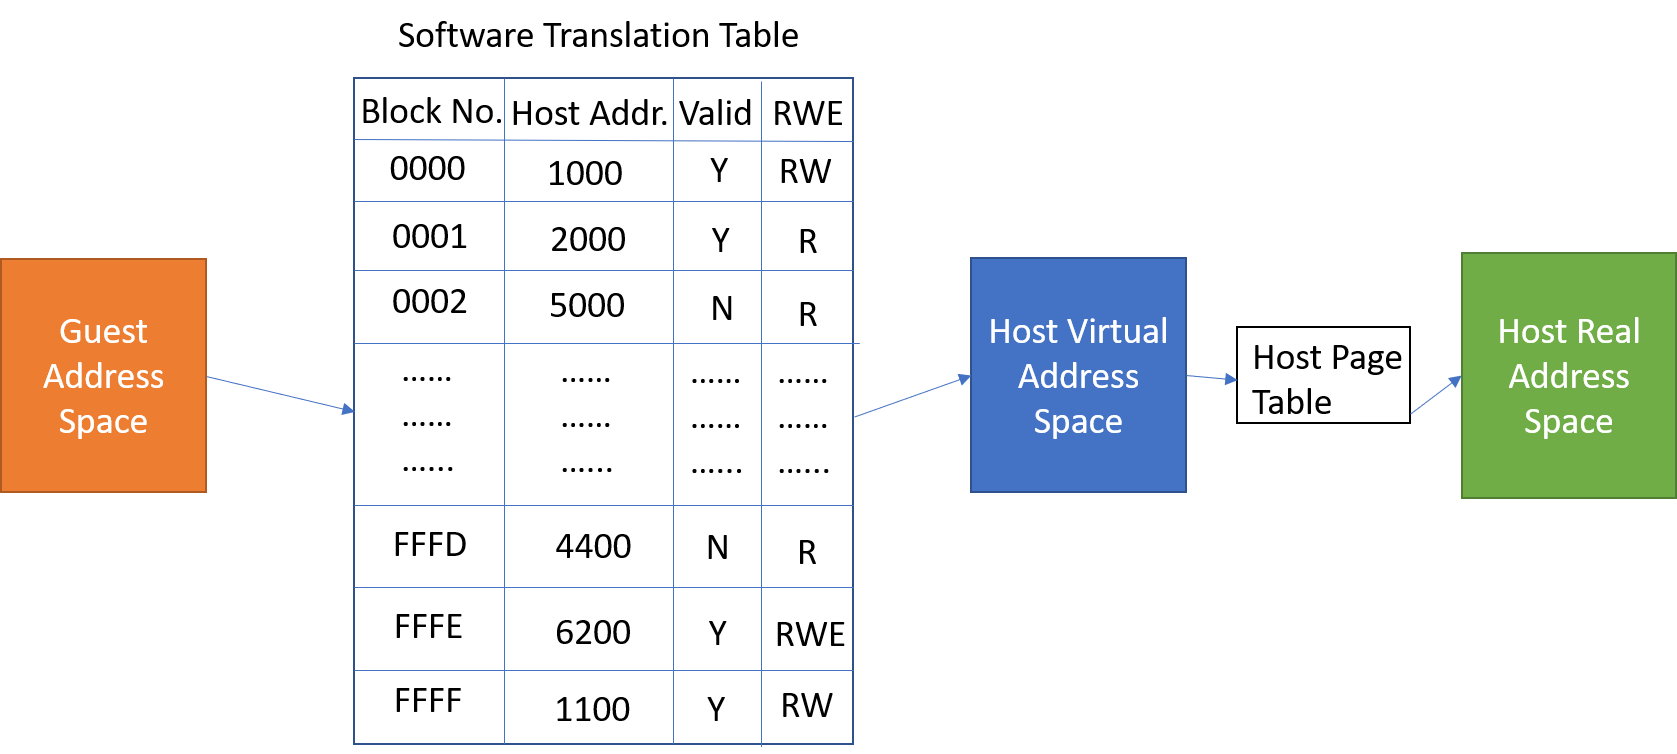
\includegraphics[scale=0.4]{2.png}
		    \end{center}
	        When guest space is non-contiguously mapped, each guest block will map to a different possibly non-contiguous host memory block with the help of above mapping table. Each entry in the table has a valid bit to indicate if the mapping is a valid mapping. The table may optionally have privilege bits if the access control has to be implemented in software by the runtime.
		    
		    
		
		\item Direct hardware translation for instruction emulation can be used,
			\begin{enumerate}
				\item When there is intrinsic compatibility at the ISA level rather than the ABI level. This is because the interface at which translation takes places is the ISA
				\item When context-free translation is preferred/required where each individual source instruction is translated to target instruction(s) (micro-ops)
				\item When the target ISA is designed specifically for source ISA thereby making the memory and register state mapping straightforward and easy
				\item When there is hardware support to set a checkpoint when each translation block is entered which can be used to restore the state at the beginning of a block during trap/exception thereby enabling precise traps
			\end{enumerate}
		
		\item Reverse translation tables are used to recover the precise source program counter (PC) of the trapping source instruction to enable the restoration of state following an exception. The table essentially consists of $<$target PC, source PC$>$ pairs.
		
		One important use case is that, It is necessary to have this table for binary translation since it does not have a continuously updated version of source PC. Also, a given target instruction may correspond to more than one source instruction (E.g. mapping a RISC ISA to CISC ISA) or the target instructions might be reorganized. In these cases, the reverse translation table helps in identifying the analyzing/interpreting the original source code to find the correct source state and PC values.
		
		\item Code cache replacement algorithm: Since the size of code cache is limited, these algorithms help in making space for new translations by removing old translated blocks from the cache. These algorithms have to consider the properties of code cache in dynamic binary optimizers which are a) fixed size, b) chaining of code blocks and c) the absence of "backing store" for storing a copy of cache contents. Some of the common algorithms are discussed below,
		
		\textbf{Flush When Full}: This algorithm lets the code cache to be filled completely and then it flushes the entire cache and starts over with an empty cache. This is a brute-force approach.
		
		Advantage: Large translation blocks are based on frequently followed control paths. However, these paths may change over time. This algorithm provides an opportunity to eliminate the stale control paths which no longer reflect the common paths in the code.
		
		Disadvantage: All blocks that are actively used before the flush have to be retranslated from scratch leading to a high translation overhead after flush.
		
		\textbf{Preemptive Flush}: This monitors the rate at which the new translations are being performed to identify a program phase change or instruction working set change. When the rate increases, the code cache is preemptively flushed to allow space for new working set code. 
		
		Advantage: Retranslation of working set is avoided in general since flush happens during the start of new working set thereby reducing the probability of cache full in the middle of a phase. 
		
		Disadvantage: Additional performance overhead is incurred in monitoring the rate of translation and triggering the flush is required. 
		
		\textbf{Fine-Grained FIFO}: The code cache is managed as a circular buffer with the oldest block being removed to have space for newest. This exploits temporal locality and is a non-brute force approach
		
		Advantage: It is a non-fragmenting algorithm and easier to implement compared to LRU since it does not have to precisely monitor the usage of each block over time.
		
		Disadvantage: Needs to keep track of chaining through backpointers to enable delinking of blocks since individual blocks are replaced. 
		
 		
%		\begin{center}
%			\begin{tabular}{|p{6.5cm}|p{6.5cm}|}
%				\hline 
%				\textbf{Advantages}  & \textbf{Disadvantages} \\
%				\hline
%				\end{tabular}
%		\end{center}    
     	
		
	        			
	\end{enumerate}
    
    \textbf{References}
    \begin{enumerate}
    	\item Jim Smith and Ravi Nair - Virtual Machines: Versatile Platforms for Systems and Processes  	
    \end{enumerate}
 

    
\end{document}